\documentclass[10pt]{article}

% Language setting
% Replace `english' with e.g. `spanish' to change the document language
\usepackage[english]{babel}

% Set page size and margins
% Replace `letterpaper' with`a4paper' for UK/EU standard size
\usepackage[a4paper,top=2cm,bottom=2cm,left=3cm,right=3cm,marginparwidth=1.75cm]{geometry}

% Useful packages
\usepackage{amsmath}
\usepackage{tikz}
\usepackage{graphicx}
\usepackage{mwe}
\usepackage{fullpage}
\usepackage{hyperref}
\hypersetup{linkcolor=blue, urlcolor=blue, colorlinks}
\usepackage{caption}
\usepackage{subcaption}
\usepackage{float}

\title{Assignment 2: \\ Programming in CUDA \\ \large \textit{Accelerator-based Programming}}
\author{Oskar Tegby}
\date{October 2022}

\setlength{\parindent}{0pt}

\begin{document}
\maketitle

\begin{tikzpicture}[remember picture, overlay]
  \node [anchor=north west, inner sep=25pt]  at (current page.north west)
     {
\includegraphics[height=3.3cm]{uu_logo.png}};
\end{tikzpicture}

\section{Introduction}
This assignment studies the computational properties of \texttt{CUDA} implementations of matrix-vector and matrix-matrix multiplication. The former is parallelized only over the rows, and the latter over both rows and columns, which is assumed to be faster than only parallelizing over the rows in the latter case. Notably, these operations are completely parallelizable since they are fully data parallel. Thus, we will dedicate this report almost exclusively to reporting and discussing the achieved bandwidth of the different implementations. Lastly, all tests are run on a \texttt{Nvidia Tesla T4} graphics card running on the \texttt{Snowy} server on the \texttt{UPPMAX} cluster. \\

The veracity of the code is tested by comparing the results for a matrix, A, and a vector, x, with strictly increasing values, since that is fully asymmetric. That is, we tested the code with e.g.
\begin{align*}
    A=
    \begin{bmatrix}
        1 & 2 & 3 & 4 \\
        5 & 6 & 7 & 8 \\
        9 & 10 & 11 & 12 \\
        13 & 14 & 15 & 16 \\
    \end{bmatrix}
    \quad\text{and}\quad
    x=
    \begin{bmatrix}
        1 \\
        2 \\
        3 \\
        4
    \end{bmatrix},
\end{align*}
as input values, which gives us the output
\begin{align*}
    b=
    \begin{bmatrix}
        30 & 70 & 110 & 150
    \end{bmatrix}.
\end{align*}
This indicates that the implementation is indeed correct.
\section{Tasks}
\subsection{Task 1}
\subsubsection{Part A}
Figure \ref{fig:mv_mult} shows the throughput of the single-precision matrix-vector multiplication run with N = M ranging from 104 to 9576 obtained by running the code with \texttt{block\_size} = 128. These results are the averages of 20 tests each run with 20 repeats to decrease the influence of computational noise, which allows us to rely on smaller details in the obtained graphs. The bandwidth is computed as
\begin{align*}
    (MN + N + M)\cdot\texttt{sizeof}(\texttt{float})\cdot 10^{-9}/t_{\text{best}}.
\end{align*}
\subsubsection{Part B}
Figure \ref{fig:mv_mult} shows a linear increase in bandwidth with the tensor sizes. The increase in bandwidth is almost exactly the double from $M=N\approx5000$ to $M=N\approx10000$. Namely, we go from about 10 GB/s to about 20 GB/s. This indicates that we are not compute-bound, as expected for such small tensor sizes.
\begin{figure}[!ht]
    \centering
    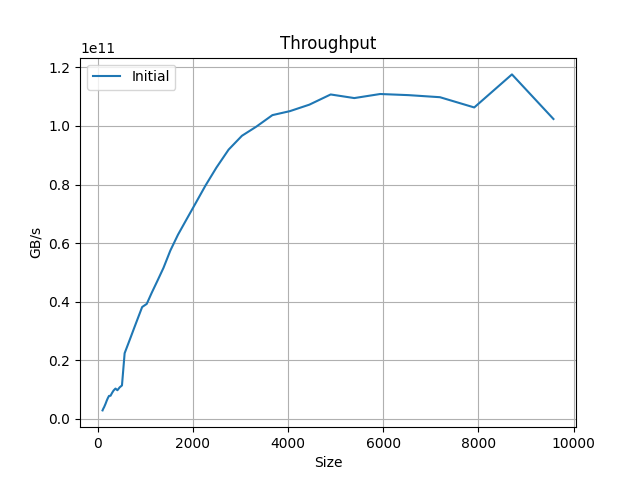
\includegraphics[width=0.8\textwidth]{figs/mv_mult.png}
    \caption{Matrix-vector multiplication with $M=N$ ranging from 100 to 10000.}
    \label{fig:mv_mult}
\end{figure}
\subsection{Task 2}
\subsection{Task 3}
\subsection{Task 4}
\end{document}
